\chapter{Technological Background}
\label{TechnologicalBackground}

\section{Hardware}
\label{Hardware}

Computer systems started with a very simple design, where a processing chip (CPU) is connected to a data storage unit (memory). The complexity of the processing chips increased, as well as the memory, specifically with the use of an hierarchy model, and current systems are usually made from multicore CPUs and various types of memory.

The most common are homogeneous systems, constituted from one or more CPU chips with their own memory bank (RAM memory) and interconnected by a specific interface, which is manufacturer-specific. Although the system uses a shared memory model, where all the data is always available for each CPU, in the case of a multiple CPU system, since the memory is distributed in one bank per CPU the system will have a Non Unified Memory Access (NUMA) pattern. This means that the access time of a CPU to a piece of memory in its memory bank will be faster than accessing memory on the other CPU bank. It is important to have the data on the CPU memory bank that the application will run to avoid the increased costs of NUMA.

With the emerging use of hardware designed for specific computing domains, hardware accelerators, which purpose is to efficiently solve a small range of problems, as opposed to general purpose CPU chips. This marked the begining of heterogeneous systems, where one or more CPU chips, operating in a shared memory environment, are accompanied by one or more hardware accelerators. The CPUs and accelerators operate in a distributed memory model, meaning that data must be explicitly passed from the CPU to the accelerator and vice-versa.

\begin{figure}[!htp]
	\begin{center}
		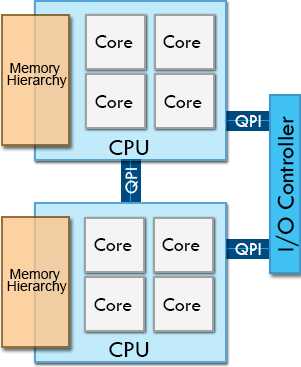
\includegraphics[scale=0.5]{../../common/img/numa_qpi.png}
		\caption{Schematic representation of a heterogeneous system.}
		\label{fig:HeterogeneousSystem}
	\end{center}
\end{figure}

Figure \ref{fig:HeterogeneousSystem} presents a schematic representation of a heterogeneous system. Note the interconnection between CPUs, responsible for the NUMA pattern, and that both CPUs must use the same interface to communicate with the hardware accelerators. This interface has a high latency for memory transfers, making it a critical spot in applications performance.

\subsection*{CPU chips}
\label{CPUChips}

Gordon Moore predicted in 1965 that for the following ten years the number of transistors on CPU chips would double every 1.5 years \cite{MooreLaw}. This was later known as the Moore's Law and it is expected to remain valid at least up to 2015. This enabled the increase in CPU chips clock frequency by the same factor as the transistors. Software developers did not expend much effort optimizing their applications and only relied on the hardware improvements to make them faster.

Due to thermal dissipation issues, the clock frequencies of CPU chips started to stall in 2005. Manufacturers shifted from making CPUs faster to increasing their throughput by adding more cores to a single chip, reducing their energy consumption and operating temperature. This marked the beggining of the multicore and parallel computing era, where every new generation of CPUs get wider, while their clock frequencies remain steady.

The CPU chips are designed as general purpose computing devices, based on a simple design consisting of small processing units with a very fast hierarchized memory attached (cache, which purpose is to reduce the slow accesses to global memory), and all the necessary data load/store and control units. They are capable of delivering a good performance in a wide range of operations, from executing simple integer arithmetic to complex branching and SIMD (single instruction multiple data, explained below) instructions. A single CPU core implements various mechanisms for improving the performance of applications, at the instruction level, with the most important explained next:

\begin{description}
	\item[\textit{ILP}] instruction level parallelism (ILP) is the overlapping of instructions, performed at the hardware or software level, which otherwise would run sequentially. At the software level it is denominated as static parallelism, where compilers try to identify which instructions are independent, i.e., the result of one does not affect the outcome of the other, and can be executed at the same time, if the hardware has resources to do so. At the hardware level, ILP can be referred as dynamic parallelism as the hardware dynamically identifies which instructions execution can be overlapped while the application is running. The three mechanisms presented next allow for ILP to be used.
	\begin{description}
		\item[\textit{Out of order execution}] is the execution of instructions in different order as they are organized in the application binary, without violating any data dependencies. This technic exposes ILP, which otherwise would not be possible.
		\item[\textit{Super Scalarity}] is a mechanism which allows dispatching a certain amount of instructions to the respective arithmetic units in each clock cycle, increasing the throughput of the CPU. Instructions that are not data dependent can run simultaneously, as long as they use different arithmetic units.
		\item[\textit{Pipelining}] is the division of an instruction execution in stages. This stages range from loading the data, instruction execution in, also pipelined, arithmetic units and writing the results back to memory. This allow, as an example, for an instruction to be loaded while other is being executed. Moreover, inside an arithmetic unit, multiple instructions can be simultaneously executed, as long as they are in different stages.
	\end{description}
	\item[\textit{Speculative execution}] is the usage of branch prediction (predict which branch of a conditional jump will be executed, before knowing the condition result), which can use complex algorithms based on previous conditional jumps, and start executing instructions in the predicted branch. If the prediction fails, the results are trashed and the other branch is executed. Current hardware is capable of executing both branches of a conditional jump and accept the one correct once the condition is resolved.
	\item[\textit{Vector instructions}] are a special set of intructions based on the SIMD model, where a single instruction is applied to a large set of data simultaneously. CPU instruction sets offer special registers and instructions that allow to take a chunk of data and execute an instruction to modify it in a special arithmetic usage. One of the most common examples is addition of two vectors. The hardware is capable of adding a given number of elements of the vectors simultaneously. This optimization is done at compile time.
	\item[\textit{Multithreading}] is the execution of multiple threads in the same core. This is possible by replicating part of the CPU resources, such as registers, and can lead to a more efficient utilization of the core hardware. If one of the threads is waiting for data to execute the next instruction, other thread can resume execution while the first is stalled. It also can allow a better usage of resources which would otherwise be idle during the execution of a single thread. If multiple threads are working on the same data, multithreading can reduce the synchronization between them and lead to a better cache usage.
\end{description}

A schematic representation of a modern CPU chip is presented in figure \ref{fig:CPUChip}. It is constituted of several, possibly multithreaded, cores, each with its own level 1 and 2 caches and a level 3 cache shared among all cores. This level 3 cache allows fast comunication and synchronization of data between cores of the same CPU.

\begin{figure}[!htp]
	\begin{center}
		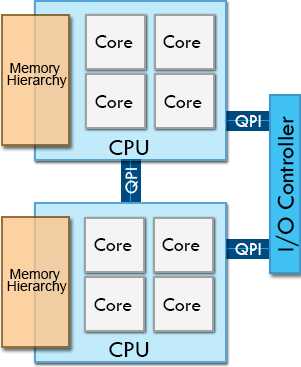
\includegraphics[scale=0.5]{../../common/img/numa_qpi.png}
		\caption{Schematic representation of a modern multicore CPU chip.}
		\label{fig:CPUChip}
	\end{center}
\end{figure}

\subsection*{Hardware Accelerators}
\label{HardwareAccelerators}

Hardware accelerators are usually made from small processing units, designed to achieve the most performance possible on specific problem domains, opposed to general purpose CPUs. They are usually oriented for massive data parallelism processing (SIMD architectures), where a single operation is performed on huge quantities of independent data, offloading the CPU from such intensive operations. Several many-core accelerator devices are available, ranging from the general purpose GPUs to the Intel Many Integrated Core line, currently known as Intel Xeon Phi \cite{Intel:MIC}, and Digital Signal Processors (DSP) \cite{Texas:DSP}. An heterogeneous platform may have one or more accelerator devices of the same or different architectures.

As of June 2013, over 50 of the TOP500’s list \cite{TOP500} are powered by any kind of hardware accelerator, which indicates an exponential growth in usage when compared to previous years. The Intel Xeon Phi is becoming increasingly popular, being the accelerator device of choice in 11 clusters of the TOP500. The most used accelerator are \nvidia GPUs.

\subsubsection*{Graphics Processing Unit}
\label{GPU}

One of the first accelerators to arrive on the market is the General Purpose Graphics Processing Unit (GPGPU). Their purpose is to accelerate image processing, which started of as simple pixel drawing and evolved to complex capabilities of 3D scene rendering, such as transforms, lighting, rasterization, texturing, depth testing, and display. They later allowed for some flexibility due to the industries demand for costumizable shaders, which also enable the possibility of using this hardware as a hardware accelerator for other purposes than image processing.



There are several accelerator devices currently arriving, or already, on the market. The first and most common are General Purpose Graphics Processing Units (GPGPUs). Recently, GPGPU makers allowed drivers to execute code that is not produced for image rendering. However, there are specific hardware details that were designed only for image rendering purposes, which limit the utilization of these devices for certain types of algorithms. One example was the use of only single precision float point arithmetic in the early GPGPUs design.

Consider GPUs and image processing as an example to justify the use of the SIMD model. Each pixel that is rendered is independent from all other pixels on the image. Their computation result from the same instructions but on different independent data, thus making their processing embarrassingly parallel. For achieving maximum performance, one important characteristic of the code, common to most accelerator device architectures, is that it needs to explore the most parallelism possible between the data to be processed, also known as data parallelism. Other device specific properties, with interest for the programmer, will be discussed later.

\subsubsection*{Intel Many Core Architecture}
\label{MIC}

\subsubsection*{Digital Signal Processor}
\label{DSP}

\section{Software}
\label{Software}

load balance
